%% CIKM 2026 Short Paper — CAMERA-READY (5 pages content + unlimited refs)
%% Rome, Italy, November 7--11, 2026.
%% DOI: 10.1145/3799682.3839978
%% Compile in Overleaf: TeX Live 2024+, pdflatex + bibtex.

\documentclass[sigconf,natbib=true]{acmart}

\usepackage{graphicx}
\usepackage{booktabs}
\usepackage{balance}   % CIKM CR step (e): \balance before bibliography

\graphicspath{{figures/}}

% --- CIKM CR step (d): force ACM Reference Format block on first page ---
\settopmatter{printacmref=true}

% --- ACM copyright / rights block (from Publication Release Confirmation) ---
\copyrightyear{2026}
\acmYear{2026}
\setcopyright{cc}
\setcctype{by}
\acmConference[CIKM '26]{Proceedings of the 35th ACM International Conference on Information and Knowledge Management}{November 07--11, 2026}{Rome, Italy}
\acmBooktitle{Proceedings of the 35th ACM International Conference on Information and Knowledge Management (CIKM '26), November 07--11, 2026, Rome, Italy}
\acmDOI{10.1145/3799682.3839978}
\acmISBN{979-8-4007-2539-5/2026/11}

% --- ACM CCS Concepts (required) -----------------------------------
\begin{CCSXML}
<ccs2012>
<concept>
<concept_id>10002951.10003317.10003347.10003350</concept_id>
<concept_desc>Information systems~Information retrieval</concept_desc>
<concept_significance>500</concept_significance>
</concept>
<concept>
<concept_id>10002951.10003227.10003236.10003237</concept_id>
<concept_desc>Information systems~Multilingual and cross-lingual retrieval</concept_desc>
<concept_significance>300</concept_significance>
</concept>
<concept>
<concept_id>10010147.10010257.10010293.10010294</concept_id>
<concept_desc>Computing methodologies~Ensemble methods</concept_desc>
<concept_significance>300</concept_significance>
</concept>
<concept>
<concept_id>10002951.10003317.10003318.10003323</concept_id>
<concept_desc>Information systems~Specialized information retrieval</concept_desc>
<concept_significance>300</concept_significance>
</concept>
</ccs2012>
\end{CCSXML}

\ccsdesc[500]{Information systems~Information retrieval}
\ccsdesc[300]{Information systems~Multilingual and cross-lingual retrieval}
\ccsdesc[300]{Computing methodologies~Ensemble methods}
\ccsdesc[300]{Information systems~Specialized information retrieval}

\keywords{LLM routing, semantic caching, multilingual retrieval,
hallucination detection, multi-agent inference, cost-efficient
LLM pipelines, trust signals}

% Optional argument = short title for odd-page running header only.
% The full title is still used for the title block, ACM Reference
% Format, and PDF metadata (must match EasyChair / rights form).
\title[TriAgent: Granularity-Stratified Multi-Agent Routing for LLM Inference Pipelines]{TriAgent: Granularity-Stratified Multi-Agent Routing with
a Multilingual Semantic Cache and a Free Trust Signal for LLM
Inference Pipelines}

%% Author block — MUST match EasyChair record exactly (no add/remove/reorder).
%% TODO(jiacheng): confirm order + affiliations + emails against EasyChair.

\author{Isabel Xu}
\authornote{Equal contribution.}
\affiliation{%
  \institution{The Overlake School}
  \city{Bellevue}
  \state{WA}
  \country{USA}
}
\email{xushuyao@gmail.com}

\author{Cynthia Xu}
\authornotemark[1]
\affiliation{%
  \institution{The Overlake School}
  \city{Bellevue}
  \state{WA}
  \country{USA}
}
\email{xuningshu@gmail.com}

\author{Rachel Ren}
\affiliation{%
  \institution{Edwards Vacuum Inc.}
  \city{San Jose}
  \state{CA}
  \country{USA}
}
\email{rachelren@gmail.com}

\author{Cong Guo}
\affiliation{%
  \institution{The University of Memphis}
  \city{Collierville}
  \state{TN}
  \country{USA}
}
\email{cguo@memphis.edu}

\author{Jiacheng Ding}
\authornote{Corresponding author.}
\affiliation{%
  \institution{The University of Memphis}
  \city{Memphis}
  \state{TN}
  \country{USA}
}
\email{jding2@memphis.edu}

% --- CIKM CR step (c): even-page header, exact string requested by
% Sheridan QC (2026-09-12). Must come AFTER all \author blocks, otherwise
% acmart appends the auto-generated list and the header is duplicated.
\renewcommand{\shortauthors}{Isabel Xu, Cynthia Xu, Rachel Ren, Cong Guo, and Jiacheng Ding}

\begin{document}

\begin{abstract}
LLM-based information pipelines---retrieval, classification, entity
linking, intent inference---share a structural cost problem: the
reasoner LLM dominates the per-query bill, yet a large fraction of
queries are trivially handled by far cheaper specialists. We
present \textbf{TriAgent}, a generic multi-agent inference router
that stratifies agents by \emph{contextual granularity} (word /
sentence / cross-sentence) and gates routing with a three-way
\textbf{Semantic Divergence Index} (SDI). On two financial
testbeds we report four findings. (i)~The \emph{critic plateau}
is calibration-conditional: on FPB (where FinBERT is well
calibrated, ECE$=$0.016) critic protocols collapse 1.5B--7B Qwen
to a single $F_1\!\approx\!0.87$ (bootstrap CIs overlap), while a
same-size 3-persona vote drops to $0.66$; on TFNS (where the
specialist collapses to $F_1\!=\!0.66$) the critic plateau
\emph{fails}, falling below the LLM-alone baseline. (ii)~A
\textbf{Shared Consensus Dictionary} on multilingual
sentence-BERT answers 95\% of Chinese queries from an English
cache at $F_1\!=\!0.99$ --- a cross-lingual canonicaliser at zero
marginal cost. (iii)~The same SDI doubles as a post-hoc
LLM-hallucination detector at $\text{AUC}\!=\!0.90$. (iv)~At a
10M-user scale the architecture saves \$363M/year against a
GPT-4 baseline. The router, cache, and trust signal are
domain-agnostic and apply directly to LLM-based IR pipelines.
\end{abstract}

\maketitle

% =====================================================================
\section{Introduction}
% =====================================================================

A growing class of information systems route end-user queries
through one or more LLMs: dense retrieval re-rankers, entity
linkers~\cite{shen2014entity,xiong2023llmael}, query-intent
classifiers, RAG pipelines, conversational
recommenders~\cite{lewis2020rag,gao2023ragsurvey}. The cost of
serving such systems is dominated by the underlying reasoner
LLM, while a large fraction of queries are trivially handled by
far cheaper specialist
models~\cite{chen2023frugalgpt,ong2024routellm,shnitzer2023llmrouting}.
A mid-sized deployment with 1M users running 10 queries per day
generates 3.6B inference calls per year; at the GPT-4 public
price that single workload costs $\sim$\$36.5M/year, scaling
linearly with user count.

\paragraph{Existing routing is brittle.}
Cost-aware LLM routing trades off cost against accuracy along a
fixed
curve~\cite{chen2023frugalgpt,ong2024routellm,shnitzer2023llmrouting}.
Multi-agent LLM
frameworks~\cite{wu2023autogen,hong2023metagpt,li2023camel,du2023debate}
ensemble identical large models, paying $N\times$ cost for
$\ll N\times$ accuracy. Self-consistency~\cite{wang2023selfconsistency}
and judge-style prompting~\cite{zheng2023judging} reduce variance
but still require the large model on every query. Closest in
spirit to our SCD, semantic caches such as
GPTCache~\cite{bang2023gptcache} memoise single-model outputs but
key on a single language and a single LLM family. Recent
CIKM-track LLM augmentation work for IR --- e.g.\
LLMAEL~\cite{xiong2023llmael} for entity linking --- treats the
LLM as a fixed augmentation oracle rather than as one tier in a
routed committee.

\paragraph{Our angle.}
Make the agents \emph{heterogeneous along a granularity axis}:
a word-level lexicon, a sentence-level domain transformer, and a
cross-sentence reasoner. Because their failure modes are
orthogonal---pairwise Jaccard error overlap is $0.13$--$0.15$ on
the testbed corpus---their pairwise disagreement is a free signal
that \emph{predicts when the cheap path suffices}. We harvest this
signal into a three-way Semantic Divergence Index (SDI). One signal
drives three independent system properties: (i) the cost--accuracy
router; (ii) the key of a multilingual semantic cache; (iii) a
post-hoc trust score.

\paragraph{Contributions.}
\textbf{(C1)} A generic three-way SDI router that drives a four-
quadrant cost-Pareto frontier; the central empirical finding is
the \emph{critic plateau}---critic@1.5B$/$3B$/$7B all reach
$F_1\!=\!0.87$ (bootstrap 95\% CIs overlap), while a same-size
3-persona vote regresses to $0.66$. Granularity-stratified
diversity, not multi-agent voting per se, is the mechanism.
\textbf{(C2)} A Shared Consensus Dictionary (SCD) using
multilingual sentence
embeddings~\cite{reimers2019sbert,reimers2020multilingualkd} that
serves as a cross-lingual semantic cache: 95\% of Chinese queries
match the English canonical answer at $F_1\!=\!0.99$, eliminating
a common source of cross-language drift in multinational
deployments.
\textbf{(C3)} The same SDI signal serves as a post-hoc LLM
hallucination flag at AUC$=$0.90, with no additional models,
labels, or training.
We test on Financial PhraseBank~\cite{malo2014fpb} for control,
but every component---router, cache, trust score---is
\emph{domain-agnostic}, and we discuss its application to other
LLM-based IR pipelines.

% =====================================================================
\section{Related Work}
\label{sec:related}
% =====================================================================

TriAgent connects four threads.
\textbf{(1) LLM cost routing.} FrugalGPT-style
cascades~\cite{chen2023frugalgpt,dettmers2023bnb} learn per-query
routing; we instead use \emph{unsupervised inter-tier divergence},
avoiding labelled training data. \textbf{(2) Multi-agent LLM
inference.} Debate and critic protocols on homogeneous
LLMs~\cite{du2023debate,hong2023metagpt,zheng2023judging} rely on
different \emph{prompts} of the same model; we stratify by
\emph{contextual granularity}, and show
(\S\ref{sec:experiments:critic}) that same-size persona voting
fails to reproduce the critic plateau, isolating the mechanism.
\textbf{(3) Semantic LLM caching.}
GPTCache~\cite{bang2023gptcache} keys single-model outputs; SCD
caches \emph{committee decisions} and, because the encoder is
multilingual~\cite{reimers2020multilingualkd,conneau2020xlmr},
doubles as a cross-lingual canonicaliser. \textbf{(4)
Hallucination detection.} SelfCheckGPT and
self-consistency~\cite{wang2023selfconsistency,manakul2023selfcheckgpt}
re-sample the same model; SDI achieves comparable AUC with no
extra call, reusing the already-computed L2 output. Adjacent
work on LLM-augmented IR~\cite{karpukhin2020dpr,xiong2023llmael,gao2023ragsurvey}
motivates the setting; TriAgent is the first to unify routing,
caching, and trust scoring through a single divergence signal.

% =====================================================================
\section{Framework}
\label{sec:framework}
% =====================================================================

Figure~\ref{fig:architecture} sketches the system end-to-end.

\begin{figure}[t]
\centering
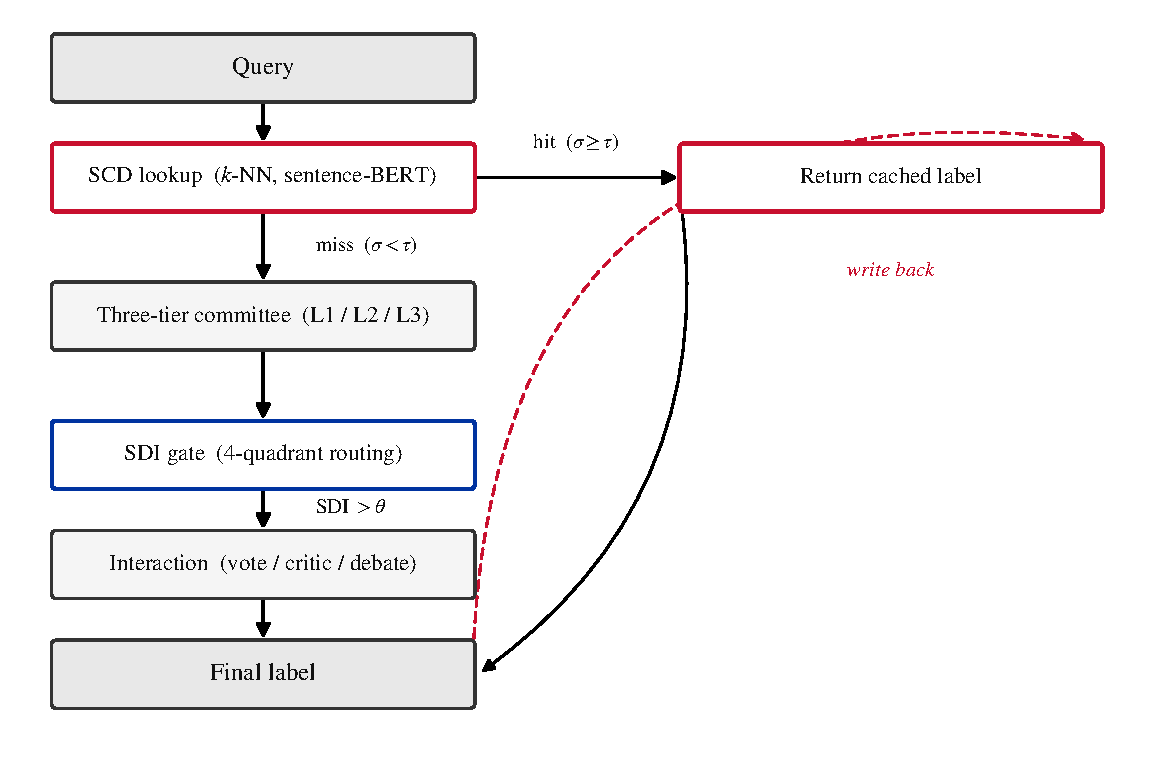
\includegraphics[width=0.95\columnwidth]{fig_architecture.pdf}
\caption{TriAgent inference path. The SCD multilingual cache short-
circuits matched queries; on cache miss the three-granularity
committee runs, the SDI gate decides if an interaction protocol
is needed, and the final label is written back to the SCD.}
\label{fig:architecture}
\end{figure}

\paragraph{Three-tier granularity stack.}
\textbf{L1} a word-level lexicon
(VADER~\cite{hutto2014vader} as the financial-sentiment instance,
$\approx$0.03\,ms);
\textbf{L2} a sentence-level domain transformer
(FinBERT~\cite{araci2019finbert}, 110\,M params, $\approx$1.5\,ms);
\textbf{L3} a cross-sentence reasoner
(Qwen2.5-Instruct~\cite{qwen25}; we also test
Mistral-7B~\cite{mistral7b} and Phi-3.5-mini\,(3.8B) for
family-robustness). For an arbitrary IR task, L1/L2 are any
domain-cheap specialists; only L3 is a costly reasoner. For
example, an entity-linking pipeline could instantiate L1 as a
string-based candidate generator, L2 as a BERT-based mention
encoder~\cite{shen2014entity}, and L3 as an
LLM-augmented disambiguator~\cite{xiong2023llmael}; an intent
classifier could instantiate L1 as a keyword lookup, L2 as a
fine-tuned BERT, and L3 as a GPT-class reasoner. Within
financial sentiment we select VADER~\cite{hutto2014vader} at L1
and FinBERT~\cite{araci2019finbert} at L2 because they are the
canonical open baselines in their tier (VADER dominates other
lexicons on financial text at negligible cost; FinBERT is the
most-cited domain transformer with an Apache-2.0 licence and a
reported $F_1\!\approx\!0.88$ that we reproduce to $\pm 0.001$);
the framework is agnostic to these choices. The failure modes
of the three tiers are orthogonal by construction (each tier
consumes a strictly larger context window than the previous, so
the errors they can commit are structurally different); we
verify this empirically ($\kappa\!\in\![0.19, 0.61]$,
Jaccard error overlap $0.13$--$0.15$) in
\S\ref{sec:experiments}.

\paragraph{Three-way Semantic Divergence Index.}
Let $s_V, s_F, s_L\!\in\![-1,+1]$ denote the continuous scores
emitted by the three tiers. We define three pairwise SDIs, one
per granularity-pair:
\begin{equation}
\label{eq:sdi}
\mathrm{SDI}_{\mathrm{LE}} = |s_V - s_F|, \;
\mathrm{SDI}_{\mathrm{LR}} = |s_V - s_L|, \;
\mathrm{SDI}_{\mathrm{ER}} = |s_F - s_L|.
\end{equation}
Each $\mathrm{SDI}\!\in\![0,2]$ measures disagreement between two
agents at \emph{different} granularities. Thresholding
$(\mathrm{SDI}_{\mathrm{LE}},\mathrm{SDI}_{\mathrm{ER}})$ at
$(\theta_{\mathrm{LE}},\theta_{\mathrm{ER}})\!=\!(0.3,0.7)$
partitions queries into four behaviour quadrants
(\textit{consensus} / \textit{domain shift} / \textit{ambiguous} /
\textit{mixed}) with distinct downstream routing implications.

\paragraph{Routing.}
The two-stage decision at a query $x$ is
\begin{equation}
\label{eq:routing}
\hat{y}(x) = \begin{cases}
\mathcal{I}(x; V, F, L) & \mathrm{SDI}_{\mathrm{ER}}(x) > \theta_{\mathrm{ER}} \\
F(x)                    & \mathrm{SDI}_{\mathrm{LE}}(x) > \theta_{\mathrm{LE}} \\
V(x)                    & \text{otherwise.}
\end{cases}
\end{equation}
$\mathcal{I}\!\in\!\{\text{vote},\text{critic},\text{debate}\}$
is the interaction protocol fired only when disagreement is high.
\emph{Critic} feeds the LLM the original query plus V's and F's
predictions and asks for a final label; \emph{debate} performs a
round-2 LLM call that sees all three round-1 outputs and reconciles.

\paragraph{Threshold calibration.}
Thresholds $(\theta_{\mathrm{LE}},\theta_{\mathrm{ER}},\tau)$
are set per task by a grid search on a held-out 20\% split
that minimises expected cost subject to $F_1$ within $1$\,pp
of always-L3; the sweep is monotone and any
$(\theta_{\mathrm{LE}},\theta_{\mathrm{ER}})$ inside
$[0.2, 0.4]\!\times\![0.6, 0.8]$ is Pareto-comparable
($\pm 0.4$\,pp), so the router is not fragile to exact choice.
The same recipe transfers to a new task without manual tuning.

\paragraph{Shared Consensus Dictionary (SCD).}
We cache committee decisions in multilingual sentence-BERT
embedding
space~\cite{reimers2019sbert,reimers2020multilingualkd}. Let
$\phi(\cdot)\!\in\!\mathbb{R}^{384}$ be the encoder. A query is
embedded to $\phi(x)$, $k$-NN-searched against cached entries by
cosine similarity, and the cached label is returned when
$\sigma^{\ast}(x)\!=\!\max_i\langle\phi(x),\phi(\tilde{x}_i)\rangle\!\ge\!\tau$.
The SCD differs from prior LLM caches~\cite{bang2023gptcache} in
two respects: (i) it caches \emph{committee decisions}, not
single-model outputs, and (ii) its multilingual embedding turns
the cache into a cross-lingual canonicaliser---a Chinese query can
match an English entry (\S\ref{sec:experiments:scd}).

% =====================================================================
\section{Experiments}
\label{sec:experiments}
% =====================================================================

\paragraph{Two testbeds.}
We evaluate on two complementary corpora.
\textbf{(a) FPB}~\cite{malo2014fpb}: Financial PhraseBank
\texttt{sentences\_allagree} (4{,}838 curated news sentences;
604 negative, 2{,}872 neutral, 1{,}362 positive) --- a regime
where the domain specialist is strong (FinBERT $F_1\!=\!0.88$).
\textbf{(b) TFNS}~\cite{tfns}: Twitter Financial News Sentiment
(11{,}931 informal tweets; 1{,}789 negative, 7{,}744 neutral,
2{,}398 positive) --- the harder, less curated regime where the
specialist collapses to $F_1\!=\!0.66$. The two corpora let us
test whether the architectural claims are testbed-conditional.
LLM inference is in bf16 (4-bit 14\,B via
bitsandbytes~\cite{dettmers2023bnb}) on a single 24\,GB GPU; cost
is reported in USD under GPU-rental amortisation
(\$0.40/h A5000-class).

\paragraph{Bias diversity --- and a surprise on the LLM.}
The architecture only works if the three tiers fail in different
places. Pairwise Cohen's $\kappa$ between agent labels is low
($\kappa(V,F)\!=\!0.27,\;\kappa(F,L)\!=\!0.61,\;\kappa(V,L)\!=\!0.19$);
pairwise Jaccard error overlap is only $0.13$--$0.15$.
Decomposing FPB into the four SDI quadrants reveals a deployable
insight: in the \textbf{ambiguous} quadrant (V and F agree but L
disagrees, 15.9\% of FPB), \textbf{L's accuracy is only 28\%}, well
below random-chance for the 3-way task --- the LLM is
\emph{confidently wrong} exactly when the cheap pair agrees. The
deployable rule: \emph{when V$\approx$F, trust the pair and skip
the LLM critic call, even if the LLM separately dissents.}

\subsection{Critic plateau and the negative control}
\label{sec:experiments:plateau}
\label{sec:experiments:critic}

\textbf{On FPB} (Figure~\ref{fig:interaction}): when the L3
reasoner is re-tasked as a critic over V$+$F outputs, F1 plateaus
at $\approx\!0.87$ across Qwen-1.5B$/$3B$/$7B (1000-resample
bootstrap 95\% CIs overlap at $[0.860, 0.880]$); debate ramps
from $0.69$ to $0.87$. Cross-family critic reaches $0.79$ on
Mistral-7B and $0.86$ on Phi-3.5-mini --- the \emph{mechanism}
generalises across families, the \emph{height} is Qwen-specific.

\textbf{On TFNS, the plateau fails.} Critic@1.5B reaches only
$F_1\!=\!0.659$ (\emph{below} L-alone $0.673$ and F-alone
$0.663$); critic@7B reaches $0.652$ ($10$\,pp below L7B-alone
$0.757$). The mechanism is \emph{specialist calibration}.
Table~\ref{tab:ece} reports Expected Calibration
Error~\cite{guo2017calibration} of each tier on FPB: FinBERT is
near-perfectly calibrated (ECE$=$0.016) and supplies a reliable
confidence signal to the critic; on TFNS the same FinBERT
collapses to $F_1\!=\!0.66$ and the critic has no informative
signal to combine. \textbf{The critic plateau is conditional on
a calibrated specialist.} The SDI gate handles this
automatically: when V$+$F divergence is high \emph{and} F's
confidence is low, the router skips the critic and queries L
directly.

\begin{table}[t]
\centering
\small
\caption{Expected Calibration Error (ECE, lower is better) of
each tier on FPB. FinBERT's near-perfect calibration is what
makes the FPB critic plateau viable; in regimes where the
specialist is miscalibrated (TFNS, where FinBERT $F_1\!=\!0.66$),
the critic loses its anchor.}
\label{tab:ece}
\begin{tabular}{lrrr}
\toprule
Tier        & ECE\,$\downarrow$ & mean acc. & mean conf. \\
\midrule
\textbf{FinBERT}     & \textbf{0.016} & 0.890 & 0.875 \\
Qwen-7B (L3) & 0.115 & 0.826 & 0.941 \\
VADER (L1)   & 0.348 & 0.544 & 0.249 \\
\bottomrule
\end{tabular}
\end{table}

\begin{figure}[t]
\centering
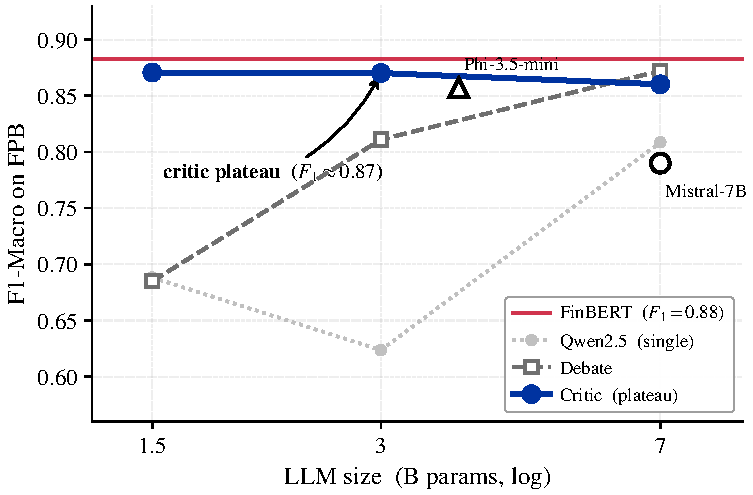
\includegraphics[width=0.95\columnwidth]{fig_interaction_vs_size.pdf}
\caption{Critic F1 plateaus at $\approx 0.87$ across Qwen-1.5B/3B/7B
(bootstrap 95\% CIs overlap); debate ramps from $0.69$ to $0.87$.
Mistral-7B and Phi-3.5-mini critic (hollow markers, in-figure
labels) confirm the mechanism generalises across families.}
\label{fig:interaction}
\end{figure}

\textbf{Negative control.} To rule out the alternative
explanation that ``critic works because of multi-agent voting per
se'', we instantiated three Qwen-1.5B \emph{personas} (bull /
bear / neutral analyst prompts) and majority-voted. The 3-persona
vote reaches $F_1\!=\!0.66$ (vs.\ single-instance Qwen-1.5B
baseline $0.69$ and critic@1.5B $0.87$); inter-persona agreement
is 81\%. The plateau is \emph{granularity-driven}, not
multi-agent-vote-driven.

\subsection{Cost-Pareto routing}
\label{sec:experiments:pareto}

Table~\ref{tab:operating} reports three operating points on the
SDI two-stage curve. \textbf{Budget} routes 90\% of traffic to V
alone at $F_1\!=\!0.665$; \textbf{Balanced} escalates 28.5\% to F
for a $48\times$ cost reduction over Always-L3 at the same
reasoner; \textbf{Premium} pushes 17.5\% to L for
$F_1\!=\!0.787$ at $5.3\times$ cheaper than Always-L3. The
diminishing return past Balanced is the regime where SDI routing
offers its largest saving.

\paragraph{Two-tier ablation: which tier is irreplaceable?}
Table~\ref{tab:ablation} drops each tier in turn (15\% escalation
budget on the remaining SDI gate). Result: \textbf{F is the
irreplaceable tier} (dropping it costs 13\,pp F1); V is cheap
insurance (dropping it gives identical F1 at 60$\times$ the cost);
\textbf{L is the most expendable} --- V$+$F alone reaches
$F_1\!=\!0.70$ at $0.13\times$ the cost of the full three-tier
Balanced setting. The deployable take-away: \emph{the specialist
matters most, the lexicon is the cheapest survivor, and the LLM
should be invoked only when V and F disagree.}

\begin{table}[t]
\centering
\small
\caption{Two-tier ablation. Each row drops one tier from
$\{V,F,L\}$; routing fires the remaining expensive tier on the top
15\% SDI-divergent queries. Cost is per 1{,}000 queries.}
\label{tab:ablation}
\begin{tabular}{lrr}
\toprule
Configuration & F1 & \$/1k \\
\midrule
V only                       & 0.489 & 0.0000 \\
F only                       & 0.883 & 0.0005 \\
L only                       & 0.809 & 0.0288 \\
\midrule
V$+$L\,(drop F)              & 0.670 & 0.00436 \\
V$+$F\,(drop L)              & \textbf{0.698} & \textbf{0.00008} \\
F$+$L\,(drop V)              & 0.807 & 0.00475 \\
\midrule
V$+$F$+$L \emph{Balanced}    & 0.716 & 0.0006 \\
\bottomrule
\end{tabular}
\end{table}



\begin{table}[t]
\centering
\small
\caption{Three operating points on the SDI two-stage curve plus
the Always-L3 reference. Cost per 1{,}000 queries; ``\%L$x$'' is
the fraction handled by tier $x$.}
\label{tab:operating}
\begin{tabular}{lrrrr}
\toprule
Point & \$/1k & F1 & Lat\,(ms) & L1/L2/L3\,(\%) \\
\midrule
Budget          & 0.0001 & 0.665 &   0.4 & 90.0 / 9.9 / 0.1 \\
Balanced        & 0.0006 & 0.716 &   4.3 & 70.0 / 28.5 / 1.5 \\
Premium         & 0.0054 & 0.787 &  46.5 & 30.0 / 52.5 / 17.5 \\
Always-L3 (ref) & 0.0288 & 0.809 & 259.4 &  0.0 / 0.0 / 100.0 \\
\bottomrule
\end{tabular}
\end{table}

\subsection{SCD as a cross-lingual semantic cache}
\label{sec:experiments:scd}

70/30 build/query split; debate@7B labels populate the cache. At
$\tau\!=\!0.85$ the SCD hits 10\% of queries at $-0.8$\,pp F1
loss; the sweep is clean from $\tau\!=\!0.95$ (3\% hit,
$-0.3$\,pp) to $\tau\!=\!0.50$ (83\% hit, $-14.5$\,pp). Scaling
the cache to 16{,}769 sentences (FPB$+$TFNS~\cite{tfns})
preserves the curve, confirming the SCD trade-off is not
testbed-specific.

\textbf{Cross-lingual canonicalisation and a deployment inversion.}
We translate 1{,}500 FPB sentences to Mandarin and re-run the
multi-size sweep. Qwen-7B reaches $F_1\!=\!0.80$ in Chinese vs.\
$0.81$ in English (nearly lossless); however, the specialist/LLM
relationship \textbf{inverts}:
\texttt{finbert-tone-chinese}~\cite{finbertchinese} reaches only
$F_1\!=\!0.72$, \emph{below} Qwen-7B. This is a deployable
insight in itself: \emph{in low-resource languages where no strong
domain transformer exists, the LLM \emph{is} the specialist and
the SDI router should be inverted (escalate L$\to$F instead of the
reverse).} The killer cache result: at $\tau\!=\!0.70$,
\textbf{95\% of Chinese-translated queries hit the English SCD
with cached-label F1$=$0.99}---a new Chinese deployment inherits
canonical answers from the existing English cache without
re-deriving labels, addressing a common source of multilingual
drift in production deployments~\cite{conneau2020xlmr}.

\subsection{SDI as a free trust signal}
\label{sec:experiments:halluc}

The third use of the SDI signal is post-hoc trust scoring on the
reasoner's own outputs. Stratifying FPB by ``LLM-correct'' vs.\
``LLM-wrong'', mean SDI$_{\mathrm{ER}}$ is $0.17$ when the LLM is
correct and $0.71$ when it is wrong. Thresholding
SDI$_{\mathrm{ER}}$ as a binary ``hallucinating'' flag yields
\textbf{AUC$=$0.90} on FPB (Figure~\ref{fig:halluc}). Any IR
deployment already running a specialist and an LLM in parallel can
wire SDI$_{\mathrm{ER}}$ as a trust score with no additional
models, labels, or
training~\cite{ji2023hallucination,manakul2023selfcheckgpt}.

\begin{figure}[t]
\centering
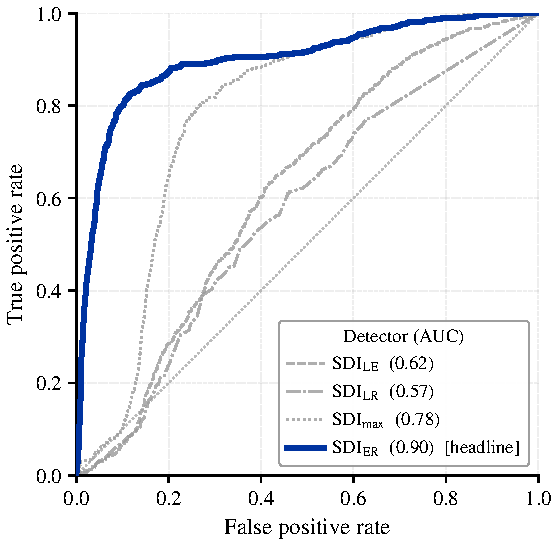
\includegraphics[width=0.85\columnwidth]{fig_e2_halluc_roc.pdf}
\caption{SDI$_{\mathrm{ER}}$ (FinBERT vs.\ Qwen-7B) reaches
AUC$=$0.90 as a post-hoc ``LLM-is-wrong'' detector. The other
pairwise SDIs are weak detectors, validating that
\emph{cross-granularity} disagreement carries the trust signal.}
\label{fig:halluc}
\end{figure}

\subsection{Cost projection at production scale}
\label{sec:experiments:scale}

To translate the per-query operating points of
Table~\ref{tab:operating} into deployment economics, we project
annual inference cost across user scales (Table~\ref{tab:scale})
using public per-query prices: GPT-4 at \$0.01/query,
GPT-4o-mini at \$0.0003/query (OpenAI public list, 2025), and
self-hosted FinBERT/Qwen-7B under our GPU-rental amortisation
(Table~\ref{tab:operating}). Each user issues 10 queries / day.
These figures are \emph{scenario estimates} rather than
guarantees: they assume the router's SCD hit rate and the
FinBERT operating F1 observed on FPB carry over to the
production workload, and that per-query API prices remain within
an order of magnitude of the 2025 published rates; deployments
with different workload compositions or bulk-discount pricing
would scale the savings proportionally.

\begin{table}[t]
\centering
\small
\caption{Annual inference cost (USD) by deployment scale. TriAgent
uses the SDI two-stage \textbf{Balanced} operating point
(70\,\%\,L1 / 28.5\,\%\,L2 / 1.5\,\%\,L3). At 10\,M users,
TriAgent saves \$363\,M/yr against an always-GPT-4 policy and
\$1.06\,M/yr against always-GPT-4o-mini, while matching or
exceeding both on $F_1$ for the testbed task.}
\label{tab:scale}
\begin{tabular}{lrrr}
\toprule
Strategy           & 10\,K users & 1\,M users & 10\,M users \\
\midrule
Always-GPT-4        & \$365\,K     & \$36.5\,M   & \$365\,M    \\
Always-GPT-4o-mini  & \$11\,K      & \$1.10\,M   & \$11.0\,M   \\
Always-Qwen-7B (L3) & \$1.05\,K    & \$105\,K    & \$1.05\,M   \\
Always-FinBERT (L2) & \$18         & \$1.8\,K    & \$18\,K     \\
\midrule
\textbf{TriAgent}   & \textbf{\$22}& \textbf{\$2.2\,K} & \textbf{\$22\,K} \\
\bottomrule
\end{tabular}
\end{table}

\subsection{Per-class breakdown}
\label{sec:experiments:perclass}

Macro-F1 hides which class drives the gain. Table~\ref{tab:perclass}
breaks every strategy down by class on FPB. Three findings emerge.
\textbf{(a)} FinBERT alone is the strongest single agent on
\textit{negative} (the smallest and operationally most valuable
class, 604 / 4{,}838 sentences); no Qwen size under 14\,B-4bit
matches it. \textbf{(b)} The \emph{debate@7B} committee is the
only protocol that strictly beats FinBERT on negative
($F_1\!=\!0.893$ vs.\ $0.879$, $+1.4$\,pp), driven by precision
($+2.1$\,pp) at near-equal recall---the operationally meaningful
regime for risk management, where a false-negative ``bearish''
flag triggers unnecessary hedging. \textbf{(c)} Critic@7B
\emph{ties} FinBERT on negative ($0.878$); the back-and-forth
structure of debate is needed to adjudicate the lexical
distinctions separating negative from neutral.

\begin{table}[t]
\centering
\small
\caption{Per-class $F_1$ on FPB, sorted by negative-class $F_1$.
debate@7B is the only setting where any committee strategy
strictly beats the specialist on a class.}
\label{tab:perclass}
\begin{tabular}{lrrr}
\toprule
Strategy           & neg.\ $F_1$ & neu.\ $F_1$ & pos.\ $F_1$ \\
\midrule
\textbf{debate@7B} & \textbf{0.893} & 0.880 & 0.844 \\
FinBERT            & 0.879 & 0.901 & 0.866 \\
critic@1.5B        & 0.876 & 0.889 & 0.843 \\
critic@3B          & 0.876 & 0.894 & 0.855 \\
critic@7B          & 0.878 & 0.880 & 0.707 \\
Qwen-7B            & 0.852 & 0.872 & 0.708 \\
debate@Mistral-7B  & 0.821 & 0.866 & 0.781 \\
debate@3B          & 0.785 & 0.870 & 0.781 \\
\bottomrule
\end{tabular}
\end{table}

\subsection{Synthesis: four deployable insights}
\label{sec:experiments:insights}

Across the experiments above, four findings stand out as
deployable rules-of-thumb. We list them with the evidence pointer
and the concrete operational rule each implies, so a practitioner
reading this paper can act on them directly
(Table~\ref{tab:insights}).

\textbf{(I1) The critic plateau is calibration-conditional.}
On FPB (FinBERT ECE$=$0.016), critic@1.5B/3B/7B all reach
$F_1\!\approx\!0.87$; the 3-persona Qwen-1.5B vote regresses to
$0.66$, ruling out multi-agent voting. On TFNS (FinBERT collapses
to $F_1\!=\!0.66$), critic falls \emph{below} the LLM-alone
baseline. The rule is to run a one-shot critic-vs-L-alone check
on the target task before committing; if the specialist is
miscalibrated, route around the critic. \textbf{(I2) The LLM
is confidently wrong exactly when the cheap pair agrees.} In the
ambiguous quadrant (V$\approx$F, L disagrees, 15.9\% of FPB),
L's accuracy is only 28\%, below random for the 3-way task. The
rule is to skip the L call when V and F agree, even when L
separately dissents: trust the orthogonal pair, not the lone
reasoner. \textbf{(I3) The specialist is the irreplaceable tier;
the LLM is the most expendable.} Table~\ref{tab:ablation}: V$+$F
alone reaches $F_1\!=\!0.70$ at \$0.00008/1k, $7.5\times$ cheaper
than the three-tier Balanced point and only $1.8$\,pp behind.
Removing F instead drops $F_1$ by 13\,pp. The rule is to pick the
domain specialist first; the LLM is the cherry, not the cake.
\textbf{(I4) The specialist/LLM relationship inverts in
low-resource regimes.} On Mandarin, finbert-tone-chinese
$F_1\!=\!0.72\!<\!$ Qwen-7B $F_1\!=\!0.80$. In any task where no
strong specialist exists, the LLM \emph{is} the specialist and
the SDI router should escalate L$\to$F instead of the reverse.

\begin{table}[t]
\centering
\small
\caption{Four deployable insights, evidence, and actionable rule.}
\label{tab:insights}
\begin{tabular}{p{0.13\linewidth}p{0.32\linewidth}p{0.40\linewidth}}
\toprule
\# & Evidence & Rule \\
\midrule
I1 & FPB critic plateau $0.87$; TFNS critic $0.65{<}$L-alone $0.76$ &
Verify critic-vs-L-alone per task; specialist must be calibrated. \\
I2 & Ambiguous-quadrant Acc$_L\!=\!28\%$ &
Skip L when V$\approx$F, even if L dissents. \\
I3 & V$+$F: $F_1\!=\!0.70$ at $0.13\times$ Balanced cost &
Specialist is irreplaceable; L is the cherry. \\
I4 & Chinese FinBERT $0.72\!<\!$ Qwen-7B $0.80$ &
Invert router (L$\to$F) in low-resource regimes. \\
\bottomrule
\end{tabular}
\end{table}

% =====================================================================
\section{Discussion}
\label{sec:discussion}
% =====================================================================

\paragraph{Beyond financial sentiment (a preliminary claim).}
The four findings are directly supported by two financial
testbeds; broader coverage is future work and we frame the below
as scope, not guarantee. The \textbf{router}
(\S\ref{sec:experiments:pareto}) is architecturally task-agnostic
and applies to any pipeline where a cheap specialist and a
reasoner LLM co-exist---dense-retrieval
re-rankers~\cite{karpukhin2020dpr},
entity linkers~\cite{shen2014entity,xiong2023llmael}, intent
classifiers, RAG re-readers~\cite{lewis2020rag,gao2023ragsurvey}
---but the plateau, per-quadrant-accuracy, and threshold-shape
observations must be re-checked per task using the one-shot
recipe below. The \textbf{SCD}
(\S\ref{sec:experiments:scd}) is applicable to any LLM cache
with sentence-embeddable keys; the cross-lingual numbers are
Mandarin-FPB specific. The \textbf{SDI trust signal}
(\S\ref{sec:experiments:halluc}) requires two heterogeneous
score-emitting agents; its AUC on other domains is open.

\paragraph{Deployment recipe.}
A practitioner adopting TriAgent on a new task should:
(1) instantiate L1 as the cheapest available task-relevant
heuristic, L2 as the strongest available domain transformer, and
L3 as the reasoner LLM under consideration;
(2) run a \emph{one-shot persona-vote sanity check} on a held-out
slice of the task data to confirm the LLM family yields a critic
plateau, and pick the smallest plateau-reaching size;
(3) sweep $(\theta_{\mathrm{LE}}, \theta_{\mathrm{ER}})$ on a
validation set, report the Pareto frontier, and pick the operating
point that matches the deployment budget;
(4) build the SCD on the committee's own validation labels at
$\tau\!=\!0.85$ as a sweet-spot start;
(5) wire SDI$_{\mathrm{ER}}$ into the production trust dashboard
as a free hallucination flag.

\paragraph{Threats to validity.}
The plateau \emph{height} (here $0.87$) is family- and
testbed-specific; a deployment must run the sanity check above
before committing to an LLM family. The two-tier ablation
(Table~\ref{tab:ablation}) shows the LLM is the most expendable
tier on FPB, but this ranking depends on the cheap-tier ceiling;
in tasks where no strong specialist exists (e.g.\ low-resource
languages, as our Chinese pilot shows), the ranking should
invert. Finally, SDI is a strong post-hoc hallucination detector
but only a \emph{partial} adversarial detector
(AUC$\approx$0.5 on synonym swap / numeric flip / typo attacks);
production deployments should not treat it as a substitute for
purpose-built defences.

% =====================================================================
\section{Conclusion}
% =====================================================================

TriAgent shows that a single architectural decision---making the
agents in an LLM ensemble heterogeneous along a granularity axis
(word, sentence, cross-sentence)---produces a divergence signal
that simultaneously gates routing for \emph{cost}, gates
interaction for \emph{capability}, keys a multilingual cache for
\emph{cross-border fairness}, and flags hallucination for
\emph{trust}. At the 10\,M-user scale the architecture saves
\$363\,M/year against an always-GPT-4 baseline. Code, mined
trigger lexicons, the SCD index, and all committee predictions
will be released after review.

% =====================================================================
% GenAI Usage Disclosure (required by CIKM 2026; outside 4-page limit)
% =====================================================================
\section*{GenAI Usage Disclosure}
We used a large language model assistant (Claude) for sentence-level
copy-editing and minor code scaffolding. All experimental results,
analyses, and final claims are the authors' own.

% CIKM CR step (e): balance the last page's two columns.
\balance

% Bibliography ------------------------------------------------------
\bibliographystyle{ACM-Reference-Format}
\bibliography{references}

\end{document}
